% !TEX TS-program = xelatex
% !TEX encoding = UTF-8

% This is a simple template for a XeLaTeX document using the "article" class,
% with the fontspec package to easily select fonts.

\documentclass[11pt]{article} % use larger type; default would be 10pt

\usepackage{fontspec} % Font selection for XeLaTeX; see fontspec.pdf for documentation
\defaultfontfeatures{Mapping=tex-text} % to support TeX conventions like ``---''
\usepackage{xunicode} % Unicode support for LaTeX character names (accents, European chars, etc)
\usepackage{xltxtra} % Extra customizations for XeLaTeX
\usepackage{titling}
\usepackage[parfill]{parskip}
\setlength{\droptitle}{-10em}
\usepackage{emptypage}


\usepackage[font=scriptsize,labelfont=bf]{caption}
%\setsansfont{Deja Vu Sans}
%\setmonofont{Deja Vu Mono}

% other LaTeX packages.....
\usepackage{geometry} % See geometry.pdf to learn the layout options. There are lots.
\geometry{a4paper} % or letterpaper (US) or a5paper or....
%\usepackage[parfill]{parskip} % Activate to begin paragraphs with an empty line rather than an indent

\usepackage{graphicx} % support the \includegraphics command and options

\title{The Role of Multi-Agent Learning in Artificial Intelligence: A new era of AI and human Interaction}
\author{Mo Afshar - Intended for Wired Magazine}
%\date{} % Activate to display a given date or no date (if empty),
         % otherwise the current date is printed 

\begin{document}
\maketitle
A multi-agent system is a computerized system consisting of multiple interacting intelligent agents within an environment. They are used to solve problems that are sufficiently difficult or regarded as impossible. Thore Graepel, a Research Scientist from Google DeepMind and Professor of Computer Science aims to give an insight of the role of multi-agent learning in Artificial Intelligence (AI) and the benefits it brings to our everyday lives. Subsequently, Google DeepMind’s goal is to ambitiously solve intelligence and to make the world a better place using AI. In this article, we will be briefly discovering what intelligence is and why multi agent systems are important. Additionally, we will briefly look at two vignettes on multi-agent learning; learning to cooperate and learning to compete.  
\par

Intelligence measures an agent’s (a program) ability to achieve goals in a wide range of environments and context. It is about solving broad set of tasks with adequate difficulty and for an agent to be able to adapt. So why exactly should we care about AI and multi-agent systems? To put it simply we live in a multi-agent world, the economy, markets, family are all systems that involve multi agency. Intelligence did not arise in isolation, there have been groups of agents, which by their interactions through different environments have brought intelligence. Moreover, these agencies compete, cooperate and communicate with each other to be successful with each other. Thus, our world is continuously evolving around programs working together to create effective systems.    
\par

Leading on, multi-agent systems provide flexibility and scalability to break down tasks into smaller sections. A good example of this which can be seen around the world is the constitution, which is broken down into legislative, executive and judicial sectors. So, living in a multi-agent world, an AI agent needs to consider the agency of others to succeed and to act to the benefit of humans. However knowing this, there are challenges along the way which need to be tackled. For example, if you look at an organisation, how do you incentivise people, and similarly for a multi-agent system, how do you provide the right reward system such that they reach a goal the system is supposed to achieve. Additionally, there can be learning problems, if you have multiple agents learning at the same time and interacting with an environment, the environment seen by the agents will be drifting, which poses challenges.   
\par

One of the important pieces on multi-agent learning is about learning to cooperate by exploring sequential social dilemmas (SSD). A social dilemma as said by Anatol Rapport is “Situations where any individual may profit from selfishness unless too many individuals choose the selfish option, in which case the whole group loses.”. An example of this can be seen in our world through pollution, public goods and the tragedy of the commons. So, by introducing SSD’s, we are essentially capturing and solving these real world social dilemmas. By using algorithms SSDs are made practical by developments in deep reinforcement learning (DRL). DRL is the paradigm of learning by trial and error, by having a rewards and punishment system and applying deep learning of neural 
networks. A neural network is simply a computer system modelled on the human brain and nervous system. Thus, by creating models using these algorithms we can see how these agents interact with each other in these environments and draw conclusions about each agent.
\par

The second vignette we will look at how to learn to compete, which is the second importance piece on multi-agent learning. This problem was explored by discovering the game of Go. Go is very difficult to play for computers as it’s search space is huge as well as it is “impossible” for computers to evaluate who is winning. This is because of the game tree complexity, as for any given position there are many positions to play. AlphaGo was created by DeepMind to solve this challenge. 
\par

\begin{figure}[h]
	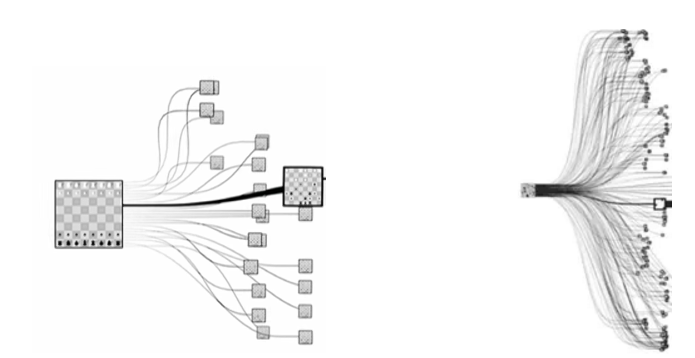
\includegraphics[width=0.8 \textwidth]{goAndChessCompare}
	\caption{The game Go has $10^{170}$ Go positions. Chess game complexity is on average 20 different moves at every stage that needs to be    		                     considered which can be viewed on the left and for the game of Go there are 300 different moves at every stage which can be viewed on the    			     right}
	\centering
\end{figure}

Thus, the idea is to use neural networks and train them to reduce the complexity of this search. Reducing the complexity is done in two ways, by creating a value network which takes a go position and returns winning probability of both the white and black positions. The second ingredient is a policy network which takes a position as input and as output gives the probability distribution over all possible moves on the board. This is the intuition of a go player. By applying the two elements, the value network reduces the depth of this search and the policy network will reduce the breadth of the search.Therefore, making AlphaGo much faster and more efficient than a human ever could. 
\par

AlphaGo was then put into test by playing against computers as well as professional Go players. In a historical match in March 2016 AlphaGo beat Lee Sedol, the best Go player in the world. This event has meant that AlphaGo has provided study material for the world’s Go enthusiasts. In conclusion, the multi-agent path towards AI is to build better AI systems such as personal health assistance and to study collective agent behaviours within the economy, the environment and much more. The ultimate aim is to help build a future where everyone benefits from AI. Finally, as grand master Gu Li has said “Together, humans and AI will soon uncover the deeper mysteries of Go”. 

\end{document}
